\documentclass[11pt,a4paper]{article}
\usepackage[utf8]{inputenc}
\usepackage{amsmath, amssymb}
\usepackage{graphicx}
\usepackage{booktabs}
\usepackage{geometry}
\usepackage{caption}
\usepackage{subcaption}
\usepackage{hyperref}
\usepackage{listings}
\usepackage{xcolor}
\geometry{margin=2.5cm}

% MATLAB listing style
\lstdefinestyle{matlab}{
    language=Matlab,
    basicstyle=\ttfamily\footnotesize,
    keywordstyle=\color{blue},
    commentstyle=\color{green!50!black},
    stringstyle=\color{red},
    numbers=left,
    numberstyle=\tiny\color{gray},
    frame=single,
    breaklines=true,
    captionpos=b
}

\title{Classification of Iris Flowers Using a Linear MSE Classifier \\[0.5em]
\large TTT4275 Estimation, Detection and Classification --- NTNU}
\author{Student A \and Student B}
\date{\today}

\begin{document}
\maketitle

%% ======================================================================
%% SUMMARY
%% ======================================================================
\begin{abstract}
This report presents the design, training, and evaluation of a linear classifier applied to the Fisher Iris dataset as part of the course TTT4275 at NTNU. The classifier is trained by minimizing the mean squared error (MSE) using iterative gradient descent. Two experiments are carried out. In the first, the effect of different training/test splits on generalization is investigated, revealing test error rates of 15--18\,\% and a notable asymmetry in misclassifications between Versicolor and Virginica. In the second, the relative importance of the four features is analyzed by progressively removing the least discriminative feature. The results show that Setosa is always linearly separable, that all four features contribute to classification performance, and that the petal measurements are the most discriminative individual features for separating the three classes.
\end{abstract}

\tableofcontents
\newpage

%% ======================================================================
\section{Introduction}
%% ======================================================================

Pattern classification is a central problem in signal processing and machine learning, where the goal is to assign an observation to one of several predefined categories based on measured features. It has broad applications ranging from medical diagnosis to speech recognition and autonomous systems.

The Iris flower dataset, originally introduced by R.~A.~Fisher in 1936~\cite{fisher1936}, is one of the most widely used benchmark datasets in classification. It consists of 150 samples from three species of Iris flowers---Setosa, Versicolor, and Virginica---each described by four measurements: sepal length, sepal width, petal length, and petal width. The dataset is known to be close to linearly separable, making it a suitable test case for evaluating linear classifiers.

In this project we design a linear classifier trained with a gradient-descent-based MSE criterion, and use it to study two aspects of the classification problem. The first is how the choice of training and test data affects classifier performance and generalization. The second is how the individual features contribute to the ability to separate the three classes linearly.

The rest of this report is organized as follows. Section~\ref{sec:theory} presents the theoretical background on linear classifiers and the MSE training criterion. Section~\ref{sec:task} describes the specific tasks to be solved. Section~\ref{sec:implementation} covers the MATLAB implementation and presents the results together with a discussion. Finally, Section~\ref{sec:conclusion} summarizes the main findings.

%% ======================================================================
\section{Theory}
\label{sec:theory}
%% ======================================================================

This section presents the theory behind the linear MSE classifier used in this project. The derivations follow the course compendium~\cite{compendium}, chapters~2.4 and~3.2.

\subsection{Linear Classifier}

A linear classifier maps a $D$-dimensional feature vector $\mathbf{x}$ to $C$ discriminant functions through a weight matrix. To incorporate a bias term, the feature vector is augmented as $\tilde{\mathbf{x}} = [\mathbf{x}^T, 1]^T \in \mathbb{R}^{D+1}$. The discriminant function for all $C$ classes is then computed as
\begin{equation}
    \mathbf{g}(\mathbf{x}) = \mathbf{W}^T \tilde{\mathbf{x}},
    \label{eq:discriminant}
\end{equation}
where $\mathbf{W} \in \mathbb{R}^{(D+1) \times C}$ is the weight matrix. A sample $\mathbf{x}$ is assigned to the class $\hat{c}$ corresponding to the largest discriminant value:
\begin{equation}
    \hat{c} = \arg\max_{c} \; g_c(\mathbf{x}).
    \label{eq:classification}
\end{equation}

\subsection{MSE Training Criterion}

The weight matrix $\mathbf{W}$ is found by minimizing the mean squared error between the classifier outputs and one-hot encoded target vectors. For $N$ training samples, the targets are arranged in a matrix $\mathbf{T} \in \mathbb{R}^{N \times C}$ where row $k$ has a 1 in column $c$ if sample $k$ belongs to class $c$, and 0 elsewhere. The MSE cost function is
\begin{equation}
    J_{\text{MSE}} = \frac{1}{N} \sum_{k=1}^{N} \left\| \mathbf{g}(\mathbf{x}_k) - \mathbf{t}_k \right\|^2 = \frac{1}{N} \left\| \tilde{\mathbf{X}} \mathbf{W} - \mathbf{T} \right\|_F^2,
    \label{eq:mse}
\end{equation}
where $\tilde{\mathbf{X}} \in \mathbb{R}^{N \times (D+1)}$ is the matrix of augmented training vectors.

\subsection{Gradient Descent}

The weights are updated iteratively using gradient descent. The gradient of $J_{\text{MSE}}$ with respect to $\mathbf{W}$ is
\begin{equation}
    \nabla_{\mathbf{W}} J_{\text{MSE}} = \frac{2}{N} \tilde{\mathbf{X}}^T \left( \tilde{\mathbf{X}} \mathbf{W} - \mathbf{T} \right),
    \label{eq:gradient}
\end{equation}
and the update rule becomes
\begin{equation}
    \mathbf{W} \leftarrow \mathbf{W} - \alpha \, \nabla_{\mathbf{W}} J_{\text{MSE}},
    \label{eq:update}
\end{equation}
where $\alpha > 0$ is the step factor (learning rate) that must be tuned so that training converges.

\subsection{Confusion Matrix and Error Rate}

Classifier performance is evaluated using a confusion matrix, which is a $C \times C$ matrix where element $(i,j)$ counts the number of samples from true class $i$ that were classified as class $j$. The overall error rate is defined as
\begin{equation}
    \text{Error rate} = \frac{\text{Number of misclassified samples}}{\text{Total number of samples}} \times 100\%.
    \label{eq:errorrate}
\end{equation}

%% ======================================================================
\section{The Task}
\label{sec:task}
%% ======================================================================

This section describes the tasks addressed in this report. The project assignment offers a choice between multiple classification problems; the Iris task is mandatory for all groups.

The Iris dataset contains 50~samples from each of three flower species (Setosa, Versicolor, Virginica), with four features per sample (sepal length, sepal width, petal length, petal width). Two sub-tasks are performed:

\textbf{Task~1 --- Training and generalization.} A linear MSE classifier is trained and tested using two different train/test splits: first using the first 30~samples per class for training and the last 20 for testing, then swapping so that the last 30 are used for training and the first 20 for testing. Confusion matrices and error rates are computed for both the training and test sets in each case, and the results are compared.

\textbf{Task~2 --- Features and linear separability.} Using the first train/test split from Task~1, histograms of each feature are plotted per class. The feature showing the most overlap between classes is identified and removed. The classifier is then retrained and tested with the remaining three features. This process is repeated, removing one more feature at each step, resulting in classifiers using 4, 3, 2, and 1 features. The confusion matrices and error rates are compared to assess the relative importance of each feature for linear separability.

%% ======================================================================
\section{Implementation and Results}
\label{sec:implementation}
%% ======================================================================

This section describes how the classifier was implemented in MATLAB and presents the results for both tasks. The full MATLAB code is provided in Appendix~\ref{app:code}.

\subsection{Implementation Overview}

The Iris dataset is provided as three separate ASCII files (\texttt{class\_1}, \texttt{class\_2}, \texttt{class\_3}), one per species, each containing 50 samples with four comma-separated feature values. The data is loaded using \texttt{load('class\_1', '-ascii')} and analogously for the other two classes. This yields three $50 \times 4$ matrices. One-hot target vectors are then constructed by assigning the appropriate column of an identity-like target matrix to each class block.

The feature vectors are augmented with a trailing 1 to incorporate the bias. Weights are initialized with small random values. Gradient descent is run for 5000 iterations with a learning rate $\alpha = 0.001$, which was found to produce stable convergence. After training, classification is performed using Equation~\eqref{eq:classification}, and the confusion matrix is computed by counting, for each true class $i$ and predicted class $j$, the number of samples where the classifier output $j$ matched or differed from the true label $i$.

Figure~\ref{fig:flowchart} illustrates the overall training and evaluation procedure.

\begin{figure}[ht]
\centering
\fbox{\parbox{0.85\textwidth}{\centering
\textbf{Flow diagram:} \\[0.5em]
Load data $\rightarrow$ Split into train/test $\rightarrow$ Augment features $\rightarrow$ Initialize $\mathbf{W}$ $\rightarrow$ \\
Gradient descent loop (5000 iterations) $\rightarrow$ \\
Classify train \& test sets $\rightarrow$ Compute confusion matrices \& error rates
}}
\caption{Overview of the training and evaluation pipeline.}
\label{fig:flowchart}
\end{figure}

\subsection{Task 1: Training and Generalization}

\textbf{Case~1} uses the first 30 samples per class for training (90 total) and the last 20 for testing (60 total). \textbf{Case~2} reverses this split.

% --- MSE convergence figure placeholder ---
% \begin{figure}[ht]
% \centering
% \includegraphics[width=0.7\textwidth]{mse_convergence.png}
% \caption{MSE convergence for Case~1 and Case~2.}
% \label{fig:mse}
% \end{figure}

\noindent\textbf{Case 1 --- Training confusion matrix:}
\begin{center}
\begin{tabular}{c|ccc}
\toprule
 & Pred.\ Setosa & Pred.\ Versicolor & Pred.\ Virginica \\
\midrule
Setosa     & 30 & 0 & 0 \\
Versicolor & 0 & 19 & 11 \\
Virginica  & 0 & 2 & 28 \\
\bottomrule
\end{tabular}
\end{center}
Training error rate: 14.44\,\%

\bigskip
\noindent\textbf{Case 1 --- Test confusion matrix:}
\begin{center}
\begin{tabular}{c|ccc}
\toprule
 & Pred.\ Setosa & Pred.\ Versicolor & Pred.\ Virginica \\
\midrule
Setosa     & 20 & 0 & 0 \\
Versicolor & 0 & 9 & 11 \\
Virginica  & 0 & 0 & 20 \\
\bottomrule
\end{tabular}
\end{center}
Test error rate: 18.33\,\%

\bigskip
\noindent\textbf{Case 2 --- Training confusion matrix:}
\begin{center}
\begin{tabular}{c|ccc}
\toprule
 & Pred.\ Setosa & Pred.\ Versicolor & Pred.\ Virginica \\
\midrule
Setosa     & 30 & 0 & 0 \\
Versicolor & 1 & 16 & 13 \\
Virginica  & 0 & 2 & 28 \\
\bottomrule
\end{tabular}
\end{center}
Training error rate: 17.78\,\%

\bigskip
\noindent\textbf{Case 2 --- Test confusion matrix:}
\begin{center}
\begin{tabular}{c|ccc}
\toprule
 & Pred.\ Setosa & Pred.\ Versicolor & Pred.\ Virginica \\
\midrule
Setosa     & 20 & 0 & 0 \\
Versicolor & 0 & 12 & 8 \\
Virginica  & 0 & 1 & 19 \\
\bottomrule
\end{tabular}
\end{center}
Test error rate: 15\,\%

\bigskip
\noindent\textbf{Comparison:}
\begin{center}
\begin{tabular}{lcc}
\toprule
 & Training Error & Test Error \\
\midrule
Case 1 (first 30 train) & 14.44\,\% & 18.33\,\% \\
Case 2 (last 30 train)  & 17.78\,\% & 15.00\,\% \\
\bottomrule
\end{tabular}
\end{center}

\textbf{Discussion.} In both cases, Setosa is perfectly classified with no errors on either set, which is expected since its petal features are well separated from the other two classes. All classification errors occur between Versicolor and Virginica.

A notable pattern is that errors are strongly asymmetric: the classifier tends to misclassify Versicolor samples as Virginica far more often than the reverse. In Case~1, 11 out of 30 training Versicolor samples and 11 out of 20 test Versicolor samples are misclassified as Virginica --- meaning over half of the test Versicolor samples are wrong. Virginica, by contrast, is classified almost perfectly. This suggests the MSE-trained decision boundary is shifted toward the Versicolor region, biasing predictions toward Virginica in the overlap zone.

An interesting observation is that Case~1 achieves a lower training error (14.44\,\%) but a higher test error (18.33\,\%) than Case~2 (17.78\,\% training, 15.00\,\% test). This shows that lower training error does not guarantee better generalization. The last~20 samples of Versicolor used as test data in Case~1 apparently lie more heavily in the overlap region, making them harder to classify. This highlights the sensitivity of small-dataset evaluation to the specific train/test split and motivates the use of cross-validation in practice.

\subsection{Task 2: Features and Linear Separability}

\textbf{Feature histograms.} Figure~\ref{fig:histograms} shows histograms of the four features for each class.

\begin{figure}[ht]
\centering
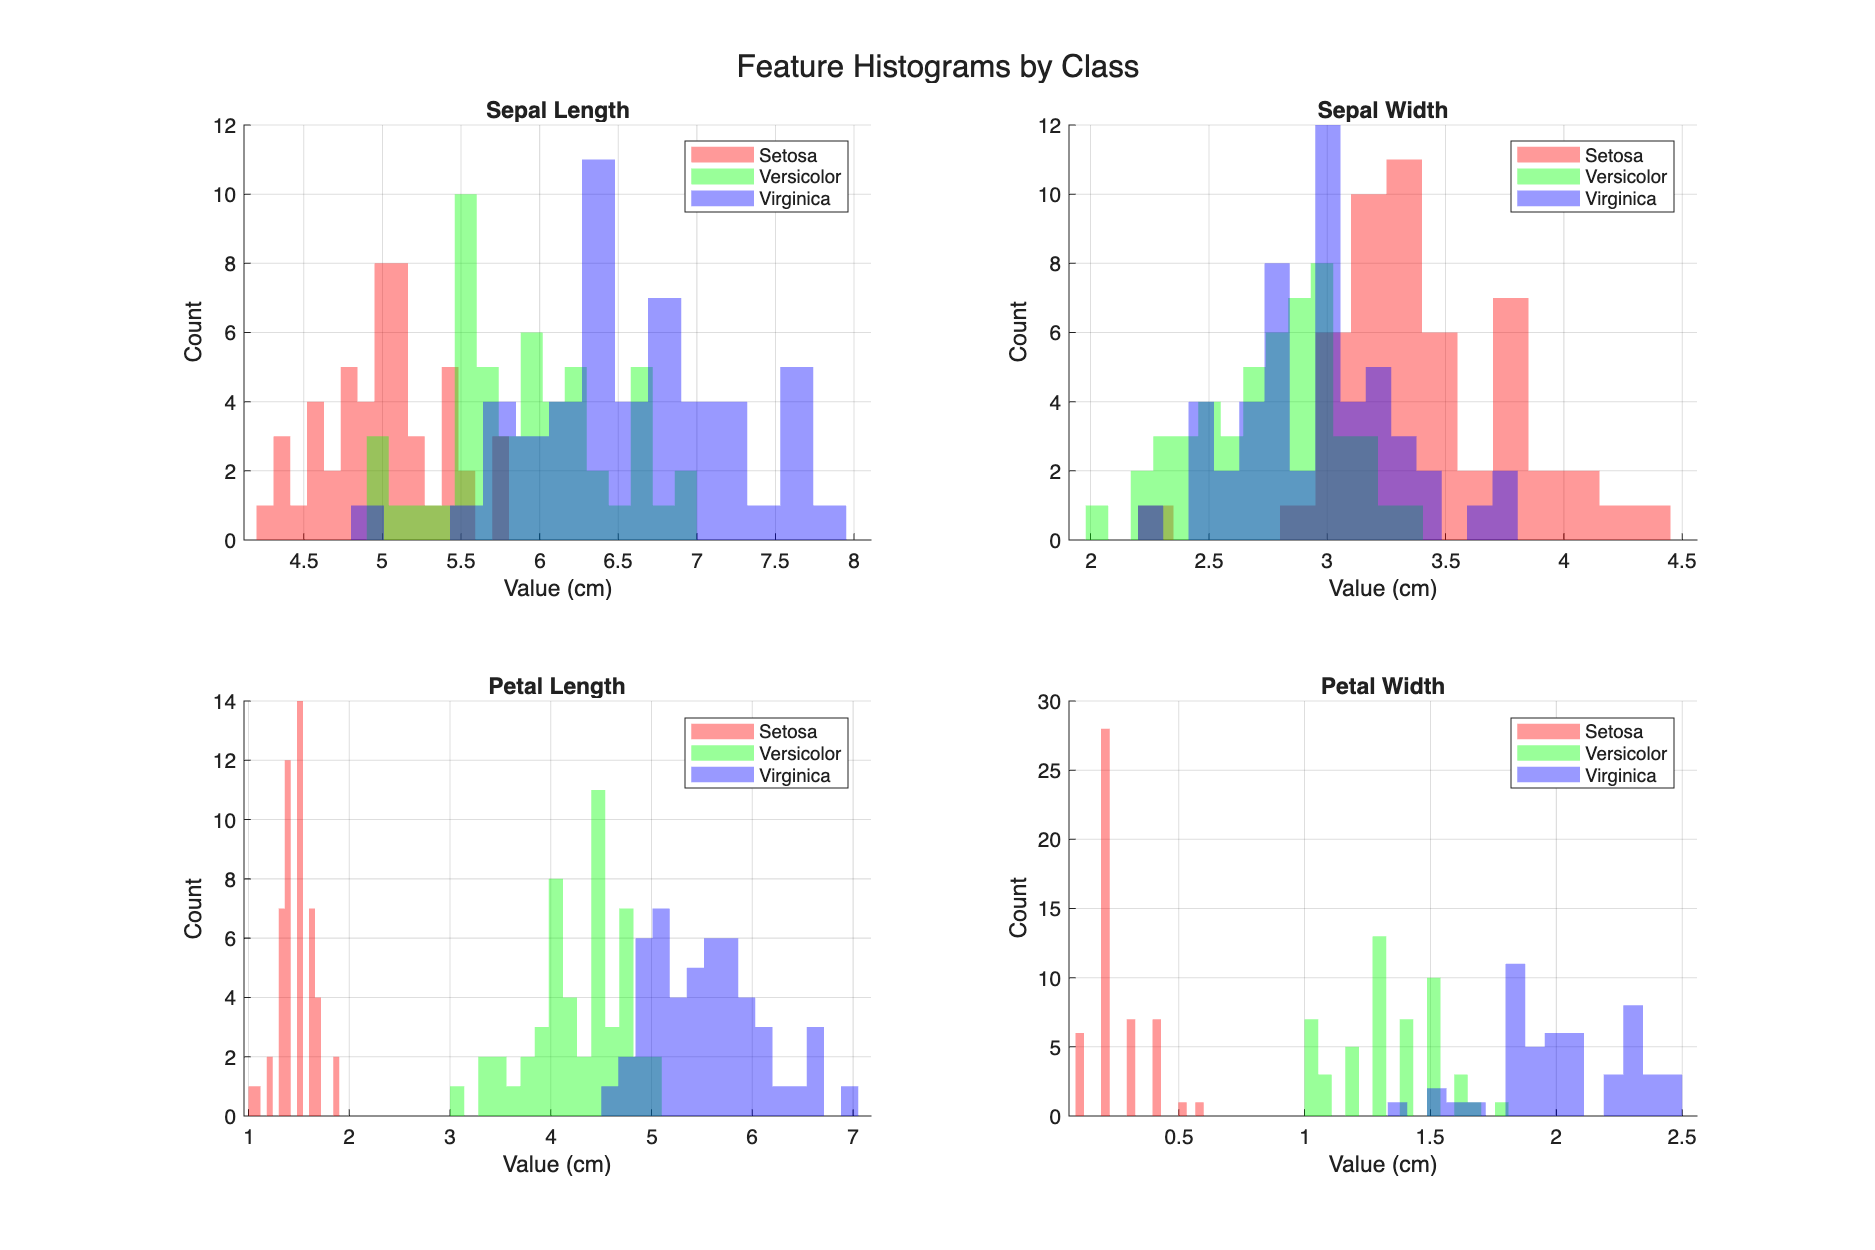
\includegraphics[width=0.9\textwidth]{feature_histograms.png}
\caption{Histograms of the four Iris features for each class. Setosa (red), Versicolor (green), Virginica (blue).}
\label{fig:histograms}
\end{figure}

From the histograms, Sepal Width shows the most overlap between all three classes and is therefore the least discriminative feature. Sepal Length also shows substantial overlap, particularly between Versicolor and Virginica. In contrast, Petal Length and Petal Width both show a clear gap between Setosa and the other two classes, with only moderate overlap between Versicolor and Virginica. Petal Length provides the best overall class separation.

Based on this analysis, the features are removed in order from most overlapping to least overlapping: Sepal Width first, then Sepal Length, then Petal Width, keeping Petal Length as the single most discriminative feature.

\bigskip
\noindent\textbf{Error rates for reduced feature sets:}
\begin{center}
\begin{tabular}{llcc}
\toprule
Experiment & Features Used & Train Error & Test Error \\
\midrule
4 features & SL, SW, PL, PW & 14.44\,\% & 18.33\,\% \\
3 features & SL, PL, PW (removed SW) & 25.56\,\% & 28.33\,\% \\
2 features & PL, PW (removed SW, SL) & 28.89\,\% & 26.67\,\% \\
1 feature  & PL only & 33.33\,\% & 33.33\,\% \\
\bottomrule
\end{tabular}
\end{center}
\textit{(SL = Sepal Length, SW = Sepal Width, PL = Petal Length, PW = Petal Width)}

\bigskip
\textbf{Discussion.} The results reveal several important properties of the features with respect to linear separability.

Using all four features gives the best performance (18.33\,\% test error). Removing Sepal Width --- the most overlapping feature according to the histograms --- causes a substantial increase in error rate to 28.33\,\% on the test set. Although Sepal Width is the least discriminative feature on its own, this result shows that it still contributes useful information in combination with the other features, helping the classifier to better separate the Versicolor--Virginica boundary in the higher-dimensional space.

Further removing Sepal Length (going from 3 to 2 features) produces only a small additional change (28.33\,\% $\rightarrow$ 26.67\,\% test error), suggesting that once Sepal Width is removed, Sepal Length provides little additional discriminative value beyond what Petal Length and Petal Width already capture.

With only Petal Length, the test error rises to 33.33\,\%, meaning one in three samples is misclassified. This demonstrates the limitation of a single feature: while Setosa remains perfectly separable in all experiments, the Versicolor--Virginica overlap along a single dimension cannot be resolved by a linear decision boundary.

Across all four experiments, Setosa is classified without any errors, confirming it is linearly separable from the other two classes regardless of which features are used. The challenge lies entirely in discriminating Versicolor from Virginica. The results show that the four features are not redundant: the full set works together to achieve the best separation, and each removed feature degrades performance, with the initial removal of Sepal Width having the largest single impact.

%% ======================================================================
\section{Conclusion}
\label{sec:conclusion}
%% ======================================================================

In this project, a linear MSE classifier was implemented in MATLAB and applied to the Fisher Iris dataset. The classifier was trained using gradient descent with a learning rate of $\alpha = 0.001$ over 5000 iterations, which produced stable convergence of the MSE cost function.

The first experiment showed that the classifier achieves test error rates of 15--18\,\%, with all errors occurring between Versicolor and Virginica --- Setosa is always perfectly classified. Errors are notably asymmetric, with Versicolor being misclassified as Virginica far more often than the reverse. The two train/test splits yielded different results: Case~1 had a lower training error but higher test error than Case~2, demonstrating that a lower training error does not guarantee better generalization. This highlights the sensitivity of evaluation to the data split and motivates the use of cross-validation.

The second experiment demonstrated that all four features contribute to classification performance, though not equally. Using all four features gives the lowest error rate (18.33\,\%), and removing even the least discriminative feature (Sepal Width) causes a notable increase to 28.33\,\%. The petal features (Petal Length and Petal Width) carry the most discriminative information individually, but the sepal features provide additional value in the full four-dimensional feature space. With only a single feature, the error rate reaches 33.33\,\%.

The project provided practical experience with implementing and evaluating a gradient-descent-based linear classifier, analyzing feature importance through histogram overlap, and understanding the limits of linear separability in a real-world dataset.

%% ======================================================================
\begin{thebibliography}{9}
\bibitem{fisher1936}
R.~A.~Fisher, ``The use of multiple measurements in taxonomic problems,'' \textit{Annals of Eugenics}, vol.~7, no.~2, pp.~179--188, 1936.

\bibitem{compendium}
TTT4275 Compendium --- Part III --- Classification, NTNU, 2025.

\bibitem{irisdata}
Iris flower data set, \url{https://en.wikipedia.org/wiki/Iris_flower_data_set}.
\end{thebibliography}

%% ======================================================================
\appendix
\section{MATLAB Code}
\label{app:code}

\subsection{Task 1: Training and Generalization}
\lstinputlisting[style=matlab, caption={iris\_task1.m}]{iris_task1.m}

\subsection{Task 2: Features and Linear Separability}
\lstinputlisting[style=matlab, caption={iris\_task2.m}]{iris_task2.m}

\end{document}